

Após as análises anteriores revelarem as dificuldades do Vidu na geração de animações 2D, o foco dos testes foi redefinido, explorando a capacidade da ferramenta em usar mais de uma imagem para a geração do vídeo. Tendo em vista que uma animação de caminhada satisfatória já havia sido obtida com a ferramenta Gemini Pro (detalhada na Seção \ref{s.ferramentaB}), o objetivo dos próximos testes no Vidu passou a ser a geração de animações com interações entre personagens, objetos e lugares. 

%outras ferramentas que possuíam uma limitação de apenas uma imagem

Além disso, uma exploração mais aprofundada da funcionalidade de referência para vídeo revelou uma forma distinta de utilização da mesma: em vez de anexar uma imagem para ser considerada como referência, a plataforma permite criar uma referência nomeada. Essa opção permite associar um nome a um conjunto de imagens de diferentes ângulos e a uma descrição, com a hipótese de que, ao fornecer à IA uma compreensão mais completa do personagem, a consistência da animação gerada poderia ser melhorada.

Primeiro, foram criadas as referências do personagem Pablo (Figuras \ref{fig:viduPablo},\ref{fig:viduPabloGeminiProSide} e \ref{fig:viduPabloGeminiProBack}), do beliche (Figura \ref{fig:viduCama}), da porta marrom (Figuras \ref{fig:viduPortaA} e \ref{fig:viduPortaB}), da porta cinza (Figuras \ref{fig:viduPortaC1} a \ref{fig:viduPortaC3}), do quarto do Pablo (Figura \ref{fig:viduQuartoPablo}) e da cena do tutorial (Figura \ref{fig:viduTutorial}). Essa criação possuía duas etapas:
\begin{itemize}
    \item Anexar imagens que representam a referência e escolhendo um nome para ela (Figura \ref{fig:viduReferenciaPablo1}); e
    \item Revisar o estilo e a descrição da referência, geradas automaticamente (Figura \ref{fig:viduReferenciaPablo2}).
\end{itemize}

\begin{figure}
    \centering
    \caption{\small Tela da primeira etapa da criação de referência do personagem Pablo no Vidu}
    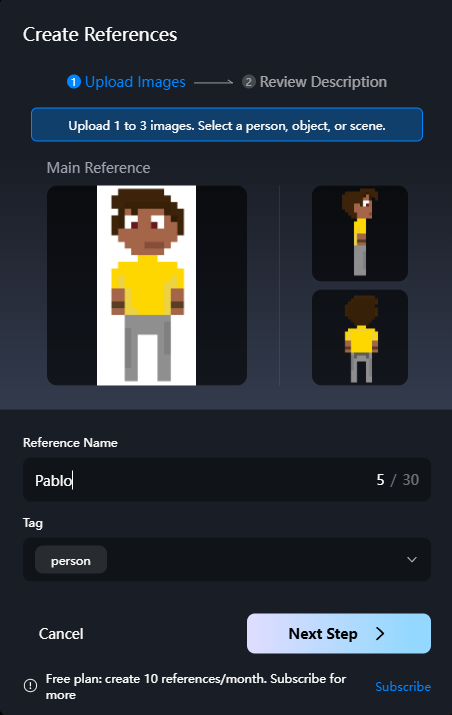
\includegraphics[width=0.3\linewidth]{figs/vidu/tela_referencia.PNG}
    \label{fig:viduReferenciaPablo1}
    \legend{\small Fonte: Elaborada pela autora.}

\end{figure}

\begin{figure}[htbp]
    \centering
    \caption{\small Tela da segunda etapa da criação de referência do personagem Pablo no Vidu}
    \label{fig:viduReferenciaPablo2}
    \begin{subfigure}{0.4\linewidth}
        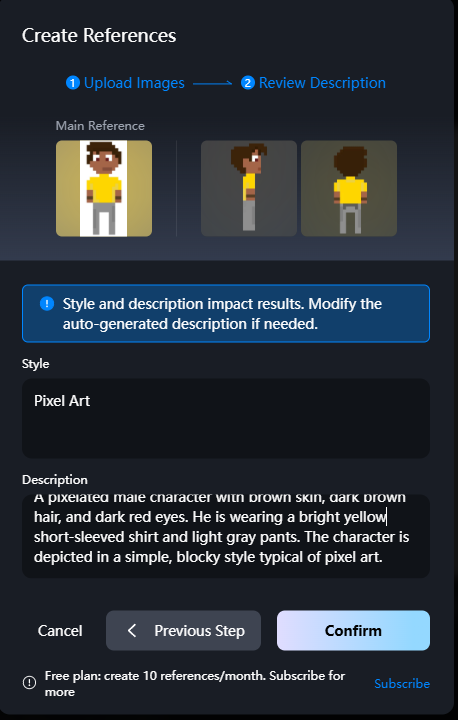
\includegraphics[width=1\linewidth]{figs/vidu/tela_referencia_2.PNG}
        \caption{\small Descrição e estilo gerados automaticamente pela IA}
        \label{fig:viduReferenciaPablo2a}
    \end{subfigure}
    \begin{subfigure}{0.4\linewidth}
        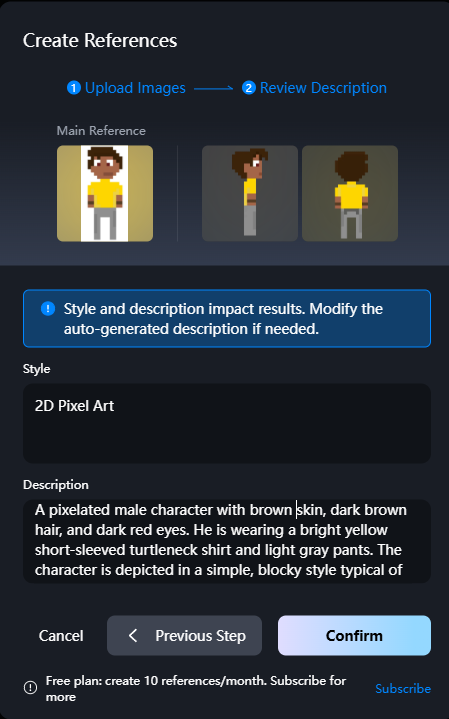
\includegraphics[width=1\linewidth]{figs/vidu/tela_referencia_2_editado.PNG}
        \caption{\small Estilo e descrição revisado manualmente, adicionando a palavra 2D no estilo e especificando o tipo de camisa na descrição}
        \label{fig:viduReferenciaPablo2b}
    \end{subfigure}
    \legend{\small Fonte: Elaborada pela autora.}
\end{figure}

As referências restantes criadas podem ser conferidas nas Figuras \ref{fig:viduReferenciaCama} a \ref{fig:viduReferenciaTutorial} no Apêndice \ref{ap.telasIA}.

Inicialmente, nessa nova bateria de testes, o objetivo era criar uma animação do personagem deitado se levantando da cama. Para isso, o nome das referências substituiu o que seria a descrição do personagem e do objeto. O resultado\footnote{\url{https://drive.google.com/file/d/1LG15atEW7Eba102-ADYkqW0z4RIYG67O/view?usp=sharing}} parecia promissor, mantendo boa parte das características do personagem e da cama, mantendo um cenário 2D e o estilo correto. Porém, ao analisar melhor o vídeo, é possível notar imprecisões no design do personagem e do beliche. O beliche gerada sofre um grande nível de zoom, cortando parte do sprite, além de que a cama debaixo possui dois travesseiros (um de cada lado) e a escada foi distorcida e movida para a lateral da cama de cima (Figura \ref{fig:viduErrosCama}). O personagem possuía características de ângulos diferentes em momentos errados, como a sua calça que ficou igual à do sprite em back view mesmo quando o personagem estava virado para frente ou para o lado (Figura \ref{fig:viduErrosPablo}). Além disso, a IA fez o personagem inicialmente sentado na cama, em vez de deitado, e apresentou frames borrados. 

\begin{figure}[htbp]
    \centering
    \caption{\small Inconsistências do beliche circuladas, em vermelho o segundo travesseiro e em azul a escada distorcida}
    \label{fig:viduErrosCama}
    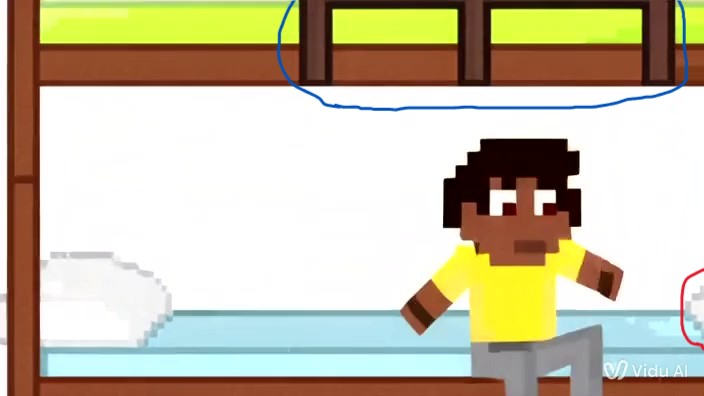
\includegraphics[width=0.7\linewidth]{figs/vidu/errosCama.jpg}
    \legend{\small Fonte: Elaborada pela autora.}
\end{figure}

\begin{figure}[htbp]
    \centering
    \caption{\small Inconsistência do personagem circulado}
    \label{fig:viduErrosPablo}
    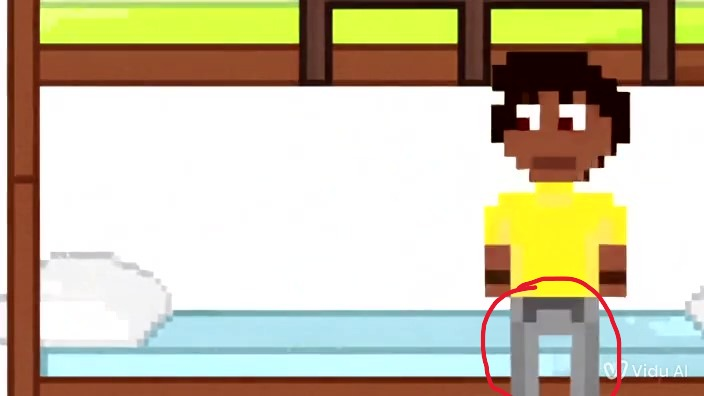
\includegraphics[width=0.7\linewidth]{figs/vidu/errosPablo.JPG}
    \legend{\small Fonte: Elaborada pela autora.}
\end{figure}

Para tentar criar a animação com o personagem realmente se levantando após estar deitado, foi feito um novo prompt especificando que o Pablo devia se deitar e, após isso, se levantar. O resultado\footnote{\url{https://drive.google.com/file/d/1PHQvJ2kcFuv2NWMyS08FiMOpw8_T9ygG/view?usp=sharing}} foi bem pior que o esperado. Apesar do personagem ter ficado mais consistente, a cama ficou muito mais incongruente, além da ação solicitada não ser gerada. O beliche foi dividida em partes e remontada como se fossem duas camas, a verde tendo virado metade verde e metade azul com dois travesseiros (Figura \ref{fig:viduErrosCama2}).

\begin{figure}[htbp]
    \centering
    \caption{\small Beliche fragmentado}
    \label{fig:viduErrosCama2}
    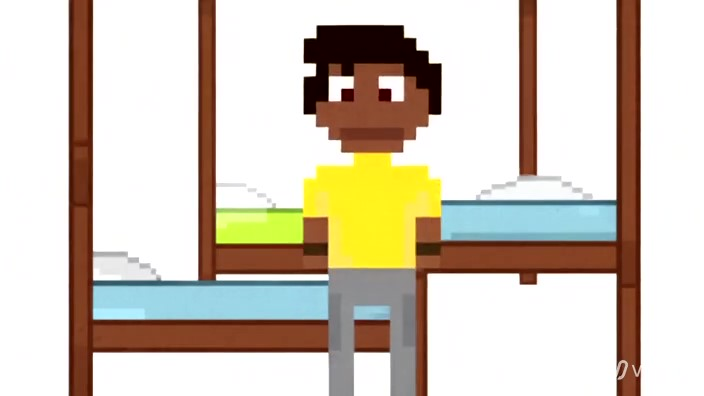
\includegraphics[width=0.7\linewidth]{figs/vidu/frame7.jpg}
    \legend{\small Fonte: Elaborada pela autora, utilizando a ferramenta Vidu.}
\end{figure}

Numa tentativa de gerar uma animação com o beliche mais consistente, foi também usado o quarto para ser o cenário da animação. A hipótese era que a falta de um fundo definido pudesse estar fazendo com que a IA modificasse a cama para ficar menos vazio o ambiente. O resultado\footnote{\url{https://drive.google.com/file/d/1PLl_ThD7HTMA2iA1j4OQ3exOZDhML5ZJ/view?usp=sharing}} gerou o personagem deitado e se levantando, porém as incongruências do beliche foram mantidas. Além disso, o quarto também não era idêntico à referência (apesar das características serem as mesmas, a forma com que elas eram desenhadas não era igual) e o personagem se teleportava de um lado para o outro na cama antes de sair dela. Esses detalhes podem ser verificados na Figura \ref{fig:viduVideoQuarto}.

%O beliche estava conectada ao beliche já existente no cenário do quarto como devia ser, mas deformou mesmo assim

\begin{figure}[htbp]
    \centering
    \caption{\small Quadro do vídeo gerado no Vidu}
    \label{fig:viduVideoQuarto}
    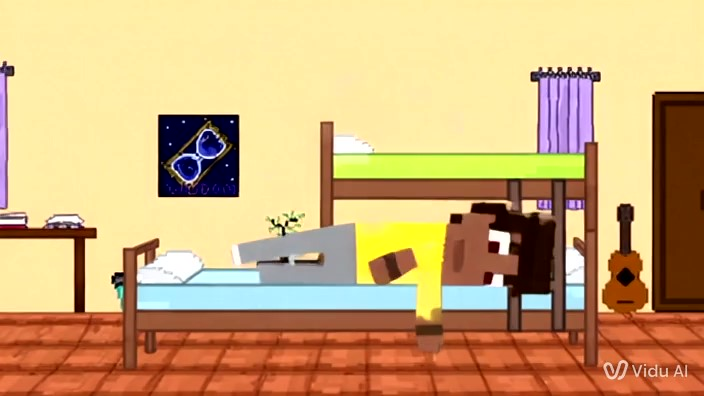
\includegraphics[width=0.7\linewidth]{figs/vidu/frame8.jpg}
    \legend{\small Fonte: Elaborada pela autora, utilizando a ferramenta Vidu.}
\end{figure}

%REVISAR SE EU CONSEGUIR IMPLEMENTAR A ANIMAÇÃO NO JOGO E MODIFICAR ELA

Em uma última tentativa utilizando apenas o personagem e a cama, o resultado\footnote{\url{https://drive.google.com/file/d/1caNcLrZhx69wZk3ShfJYDh1qzkkP57Zo/view?usp=sharing}} apresentou uma melhora significativa. Embora ainda apresentasse inconsistências, como uma leve mudança de perspectiva da cama e o personagem deslizando antes de iniciar o movimento, a estrutura do beliche foi gerada com maior precisão, e a ação principal de levantar-se foi executada.

Apesar de ter sido a melhor animação produzida pela ferramenta até o momento, o resultado ainda exigiria um processo de edição manual extenso para ser considerado satisfatório, incluindo a potencial remoção do beliche para ajustar a animação do personagem diretamente no cenário do jogo. Considerando que o esforço de modificação seria desproporcional à importância desta animação para o projeto, optou-se por não editar ou implementar o resultado final.

Na bateria de testes seguinte, o objetivo foi produzir uma animação do personagem abrindo a porta. Por causa dos erros de consistência do personagem nos vídeos anteriores, foi adicionada na descrição do Pablo uma parte especificando o ângulo de cada imagem (Figura \ref{fig:viduReferenciaPabloEditado} do Apêndice \ref{ap.telasIA}). 

Os resultados\footnote{\url{https://drive.google.com/drive/folders/1aWPXy7SAJmMUJlEvNTxy2__ntK6ZjZy6?usp=drive_link}} apresentaram ou deformações na porta (Figura \ref{fig:viduPortaChao}) ou imprecisões na animação da abertura dela (Figura \ref{fig:viduPortaAbrindo}). Apesar do movimento em específico do personagem ser adequado, é possível encontrar quadros onde ele possui incongruências (Figura \ref{fig:viduDoisBraceletes}) e a alta taxa de frames deformados ainda continua. A interação completa pode ser consultada nas Figuras \ref{fig:vidu10} a \ref{fig:vidu12} do Apêndice \ref{ap.telasIA}.

% sem fundo = distorce porta
%descrição fundo ou quarto fundo = porta consistente


\begin{figure}[htbp]
    \centering
    \caption{\small Porta deformada para fazer o chão no vídeo gerado pelo Vidu}
    \label{fig:viduPortaChao}
    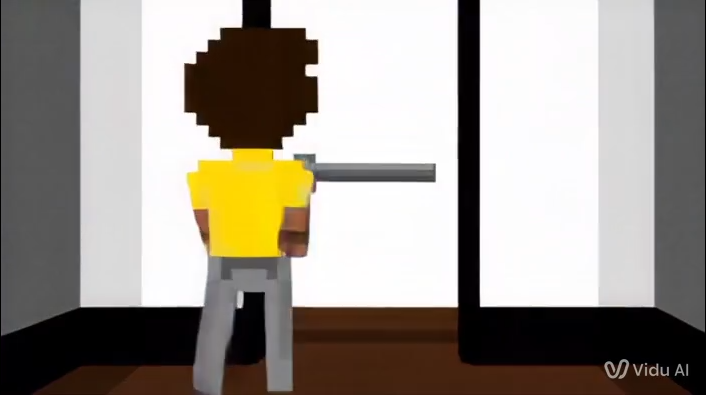
\includegraphics[width=0.6\linewidth]{figs/vidu/porta_deformada.PNG}
    \legend{\small Fonte: Elaborada pela autora, utilizando a ferramenta Vidu.}
\end{figure}

\begin{figure}[htbp]
    \centering
    \caption{\small Porta abrindo pelo lado errado no vídeo gerado pelo Vidu}
    \label{fig:viduPortaAbrindo}
    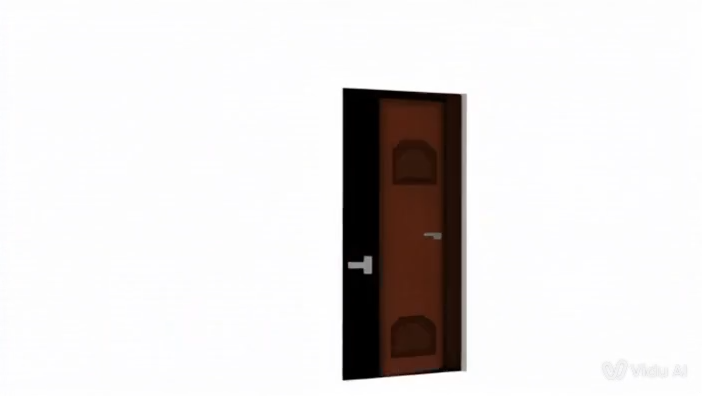
\includegraphics[width=0.7\linewidth]{figs/vidu/porta_abrindo_lado_oposto.PNG}
    \legend{\small Fonte: Elaborada pela autora, utilizando a ferramenta Vidu.}
\end{figure}

\begin{figure}[htbp]
    \centering
    \caption{\small Dois braceletes no braço do personagem no vídeo gerado pelo Vidu}
    \label{fig:viduDoisBraceletes}
    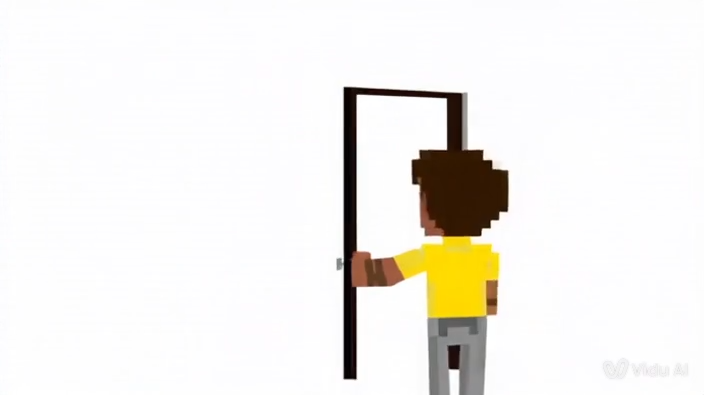
\includegraphics[width=0.7\linewidth]{figs/vidu/Braceletes.PNG}
    \legend{\small Fonte: Elaborada pela autora, utilizando a ferramenta Vidu.}
\end{figure}

Comparando as baterias de testes, notou-se que foi gerada a mesma área parcial do cenário nos testes em que o quarto foi utilizado, mesmo que a referência tivesse mais partes. Além disso, o beliche foi desenhado no mesmo lugar onde estava localizado no quarto, enquanto a porta foi posicionada numa região completamente distinta. 

Com a análise comparativa foi criada uma hipótese sobre o comportamento da IA: ela parece processar apenas a área central da imagem de referência do cenário. Como a beliche estava posicionada perto do centro da imagem do quarto, sua localização no vídeo foi correta. A porta, no entanto, que estava na borda da imagem de referência, foi cortada de sua posição original e gerada incorretamente no centro da cena.


\begin{figure}[htbp]
    \centering
    \caption{\small Comparação da geração dos objetos em relação ao quarto no Vidu}
    \label{fig:viduComparaLugar}
    \begin{subfigure}{0.4\linewidth}
        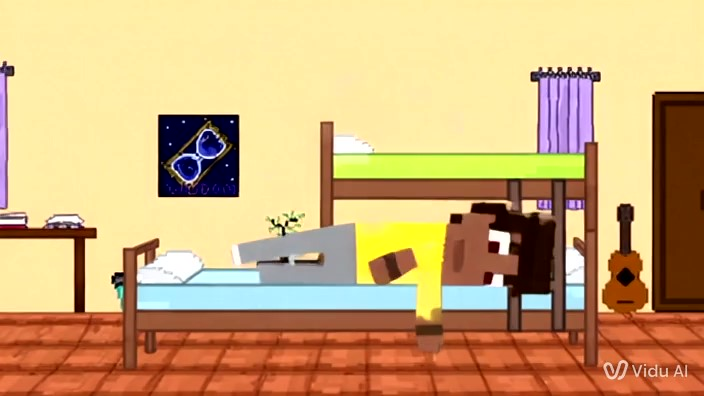
\includegraphics[width=1\linewidth]{figs/vidu/frame8.jpg}
        \caption{\small Beliche inconsistente posicionada no lugar correto}
        \label{fig:viduComparaBeliche}
    \end{subfigure}
    \begin{subfigure}{0.4\linewidth}
        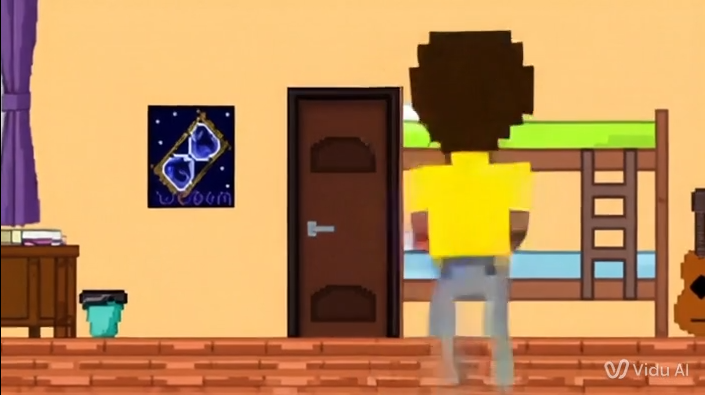
\includegraphics[width=1\linewidth]{figs/vidu/frame11.PNG}
        \caption{\small Porta consistente posicionada no lugar incorreto}
        \label{fig:viduComparaPorta}
    \end{subfigure}
    \legend{\small Fonte: Elaborada pela autora.}
\end{figure}

Em busca de tentar aprimorar os resultados, foi encontrada uma técnica mais complexa de criar prompts para a ferramenta do Vidu. Para gerar vídeos mais consistentes e unificados, foi necessário: destacar o estilo artístico, usar termos precisos e simples, descrever o sujeito, a cena e o ambiente, e utilizar palavras-chave atmosféricas \cite{docs_2025}. Dessa forma, um novo prompt foi idealizado (Figura \ref{fig:vidu13} do Apêndice \ref{ap.telasIA}), gerando um vídeo\footnote{\url{https://drive.google.com/file/d/1o_BNadSvUQ5w4TaJZ5DBUaw0V66rc-na/view?usp=sharing}} melhor que os anteriores. Os sprites não possuem inconsistência notável em relação à referência e a porta abre de maneira precisa, porém o personagem só segura a maçaneta após a porta abrir, além de que ela começou aberta e depois repentinamente tornou-se fechada. A animação da porta abrindo foi satisfatória, mesmo que o movimento do personagem para abri-la não tenha sido. Apesar disso, outra ferramenta foi capaz de gerar uma animação da mesma qualidade para a porta e com menos necessidade de edições porque o personagem não estava cobrindo parte do objeto.

Ainda usando essa nova estratégia de prompt, no próximo teste o objetivo passou a ser produzir uma animação do personagem pulando. Para isso foi utilizada apenas a imagem em side view em vez da referência Pablo, com o objetivo de evitar erros em que o personagem vira o corpo em outro ângulo no meio da animação. Os vídeos\footnote{\url{https://drive.google.com/drive/folders/1Lpi7zzY0BvaPkgjSv7xvc5aVubXCEVor?usp=drive_link}} criados não alcançaram as expectativas, renderizando um fundo branco e preto e fazendo com que o personagem parecesse estar caindo ou apenas pulando de um pé só. Além disso, essa animação específica demonstra uma grande taxa de quadros borrados, ainda maior do que o esperado. Interação pode ser consultada na Figura \ref{fig:viduPulo1} no Apêndice \ref{ap.telasIA}.

Também tentou-se criar uma animação para a porta abrindo, só que dessa vez em side view e sem a presença do personagem. Os resultados\footnote{\url{https://drive.google.com/drive/folders/1oplBZG15V_LfexCUw-X973PXb3gNfzIP?usp=drive_link}} não foram suficientes, sem produzir o movimento da porta abrir na visão correta, girando-a e até mesmo duplicando-a. Processo demonstrado nas Figuras \ref{fig:viduPorta1} e \ref{fig:viduPorta2}.

Em geral, essa funcionalidade da ferramenta apresentou grande potencial, porém possui uma grande queda de qualidade para gerar animações especificamente 2D, além de apresentar alguns erros de consistência e precisão. Esse método consegue fornecer uma base para a animação ser modificada manualmente, corrigindo diversos detalhes.

